%\documentclass[12pt]{article}
\documentclass[sigconf]{acmart}

\usepackage{booktabs} % For formal tables
\usepackage{xspace}
\usepackage[]{algorithm2e}
\usepackage{verbatim}

%\fancyhf{} % Remove fancy page headers 
%\fancyhead[C]{Anonymous Submision \#517 to ACM CCS 2017} \fancyfoot[C]{\thepage}

%\fancyhead{}
%\settopmatter{printacmref=false, printfolios=false}

% Copyright
%\setcopyright{none} % No copyright notice required for submissions
%\acmConference[Anonymous Submission to ACM CCS 2017]{ACM Conference on Computer and Communications Security}{Due 19 May 2017}{Dallas, Texas}

\copyrightyear{2017} 
\acmYear{2017} 
\setcopyright{acmlicensed}
\acmConference{CCS '17}{October 30-November 3, 2017}{Dallas, TX, USA}\acmPrice{15.00}\acmDOI{10.1145/3133956.3134033}
\acmISBN{978-1-4503-4946-8/17/10}

%\usepackage{titling}
\usepackage{color}
\usepackage{float}
\usepackage{graphicx}
\graphicspath{ {images/} }
\usepackage{subcaption}
\usepackage{dblfloatfix}
%\usepackage{fixltx2e}
\usepackage{tikz}
\usetikzlibrary{arrows}
\usetikzlibrary{positioning}
\usetikzlibrary{patterns}
\usepackage{pgf-umlsd}
\usepgflibrary{arrows}
%\usepackage{pgfplots}
%\pgfplotsset{width=10cm,compat=1.9}
%\usepgfplotslibrary{external}
%\tikzexternalize
\usepackage{flushend}

\usepackage{listings}
\newcommand{\code}[1]{\lstinline|#1|}
\newcommand*\LSTfont{\footnotesize\ttfamily\SetTracking{encoding=*}{-60}\lsstyle}
\lstset{
        language=Java,
        xleftmargin=14pt,
        numbers=left,
        basicstyle=\LSTfont,
        numberstyle=\color{gray}\LSTfont,
        keywordstyle=\color{blue}\LSTfont,
        commentstyle=\color{darkgreen},
        morekeywords={*,Push,Call,GasLimit,BlockTimestamp,BlockNumber,GasLimit,GasPrice,Balance,BlockHash,Difficulty,MessageField,MessageCaller, Add, Mul, Sub, Address, Caller, MStore, MLoad, SStore, SLoad, Jump, JumpI,JumpDest, Stop, CallValue,LT,EQ,NOT,SHA3,CoinBase,Swap1,Dup1,Log0,Pop,Push1,Push2,Push32,MStore8,contract,uint,function,call,bool,public},
        numbersep=5pt,
        frame=none,
        firstnumber=auto,
        escapeinside={(*@}{@*)},
        captionpos=b,
}
\lstdefinelanguage
   [evm]{Assembler}     % add a "evm" dialect of Assembler
   [x86masm]{Assembler} % based on the "x86masm" dialect
   % with these extra keywords:
   {morekeywords={PUSH4, PUSH2, JUMPI, CALLDATALOAD, JUMP, JUMPDEST, DUP, SWAP}} % etc.



\newcommand{\name}{\textsc{Revive}\xspace}
\definecolor{darkred}{rgb}{0.75,0,0}
\newcommand{\todo}[1]{{\bf \color{darkred}$\blacktriangleright$#1$\blacktriangleleft$}}

\title{\name: Rebalancing Off-Blockchain Payment Networks}
%\subtitle{test}
\date{}

\author{Rami Khalil}
\affiliation{%
  \institution{Department of Computer Science\\ETH Zurich, Switzerland}
}
\email{rkhalil@student.ethz.ch}

\author{Arthur Gervais}
\affiliation{%
  \institution{Department of Computer Science\\ETH Zurich, Switzerland}
}
\email{arthur.gervais@inf.ethz.ch}

\renewcommand{\shortauthors}{Khalil and Gervais}

\keywords{ACM proceedings, \LaTeX, text tagging}

\makeatletter
\newenvironment{figurehere}
{\def\@captype{figure}}
{}
\makeatother

\begin{document}

\begin{abstract}
Scaling the transaction throughput of decentralized blockchain ledgers such as Bitcoin and Ethereum has been an ongoing challenge. Two-party duplex payment channels have been designed and used as building blocks to construct linked payment networks, which allow atomic and trust-free payments between parties without exhausting the resources of the blockchain.

Once a payment channel, however, is depleted (e.g., because transactions were mostly unidirectional) the channel would need to be closed and re-funded to allow for new transactions. Users are envisioned to entertain multiple payment channels with different entities, and as such, instead of refunding a channel (which incurs costly on-chain transactions), a user should be able to leverage his existing channels to rebalance a poorly funded channel.

To the best of our knowledge, we present the first solution that allows an arbitrary set of users in a payment channel network to securely rebalance their channels, according to the preferences of the channel owners. Except in the case of disputes (similar to conventional payment channels), our solution does not require on-chain transactions and therefore increases the scalability of existing blockchains. In our security analysis, we show that an honest participant cannot lose any of its funds while rebalancing. We finally provide a proof of concept implementation and evaluation for the Ethereum network.
\end{abstract}

\maketitle

\section{Introduction}
Permissionless blockchains such as Bitcoin and Ethereum, where any participant can choose to join and leave at any moment, have allowed to replace a trusted third party with a network of mutually mistrusting peers. Besides the transfer of monetary value, Ethereum supports the execution of smart contracts, Turing complete code which is executed in consensus among all peers of the network.

One of the main costs of the decentralization of permissionless blockchains is their performance. In its current state, Bitcoin for example only supports up to 7 transactions per second --- clearly insufficient to grow to a mainstream payment system. Because the simple re-parametrization of permissionless blockchains has shown to not solve the scalability performance beyond 100 transactions per second~\cite{gervais2016security}, and alternative consensus mechanisms typically introduce different trust assumptions~\cite{luu2015scp,kogias2016enhancing,eyal2016bitcoin,pass2016hybrid}, second layer payment channels~\cite{lightning, sprites, raiden, flare} have been introduced.

%Essentially each transaction reflects a change of balance in the ledger, and due to the decentralized nature of the ledgers, each transaction takes a significant amount of time to be safely completed. As these cryptocurrencies grow in popularity, they need to scale to meet the increasing usage demands put on them. As of yet, the transaction throughputs of Bitcoin and Ethereum hover around tens of transactions per second, which is orders of magnitude slower than what centralized ledgers such as those backing payment processors such as Visa and Mastercard can support.

%With the goal of increasing processing efficiency, secondary "off-chain" payment protocols have been suggested. 
Payment channels aim to establish direct peer-to-peer payment channels that allow two parties to privately maintain and update a two-party ledger. The benefit is that their individual transactions are not required to be written to the blockchain, while keeping a guarantee of being able to claim their rightful funds in the global blockchain ledger at any given time. Payment channels have a few limitations, but should improve the transaction throughput of a decentralized ledger to the network bandwidth of the two peers participating in a payment channel.

Payment networks~\cite{lightning, raiden} allow to perform payments between parties that are not immediately connected by a payment channel. These linked payments utilize a chain of payment channels as intermediate links between two parties that wish to transact with each other off-chain, without having to open a new payment channel or conduct an on-chain transaction. Several contributions aim to improve the performance characteristics of payment networks. Sprites~\cite{sprites}, for example, aims to address the worst-case completion time of an off-chain linked-transaction. Flare~\cite{flare} proposes routing strategies that aim to optimize the amount of time taken on average to find a payment route.

%Multiple designs for payment channels have been proposed~\cite{raiden, lightning, sprites}, each with its own set of mechanisms and trade-offs. 
%In this work, we mainly focus on designs that allow indirect, or linked, payments between parties that are not immediately connected by a payment channel.
%Off-chain payment protocols, such as the lightning \cite{lightning} and raiden \cite{raiden} networks, allow to move the burden of transaction settling from the blockchain to the two or more participating peers. 

%Several new proposals have surfaced the literature that aim to improve the worst-case completion time of an off-chain transaction, such as in \cite{sprites}, or the scalability of blockchain payments, as in \cite{scale}.

One fundamental flaw of existing payment channels however remains the inability to refund a payment channel \emph{without} performing transactions on the blockchain. Once a payment channel is depleted, the channel needs to be closed and re-funded, requiring at least two expensive on-chain transactions. Before refunding a channel, users might first opt to choose more expensive channel routes, which will increase the transaction costs over payment channels (each hop in a payment network receives a relay fee).

\paragraph{This work} In this work, we propose to the best of our knowledge the first rebalancing scheme for off-chain payment networks. Our solution enables a set of members in a payment network to shift balances between their payment channels safely. Rather than to enact previously mandatory on-chain channel closing and re-opening, our solution allows participants to safely \name a channel by reallocating off-chain the funds they have assigned to their payment channels. Rebalancing is naturally limited by certain restrictions on how much can be reallocated, because we do not shift the deposits made within a payment channel but rather the credits that participants are entitled to. In our security analysis, we show that an honest participant is guaranteed not to lose any of its funds while rebalancing.
%\paragraph{This work} In this work, we propose to the best of our knowledge the first rebalancing scheme for off-chain payment networks, that enables a set of members in a payment network to safely shift balances between their payment channels. Rather than to have to enact on-chain channel closing and re-opening, our solution allows participants to safely \name a channel by reallocating the funds they have assigned to their payment channels. The rebalancing is performed off-chain, with certain restrictions on how much can be reallocated. \name therefore allows to enable payment networks to redistribute the funds in their off-chain ledgers so as to optimize away any skewed payment channels that may lead to longer, more costly payment routes being chosen.

The main contributions of our work are as follows:
\begin{itemize}
\item To the best of our knowledge, \name is the first rebalancing scheme for payment channels, that allows a user to utilize any other of his channels for rebalancing a particular channel.
\item If all participants of the rebalancing are responsive (i.e.\ honest), rebalancing with \name is \emph{free}. \name thus increases the transaction scalability of permissionless blockchains by reducing the frequency at which on-chain channel refunding is necessary. Simultaneously, \name reduces the costs of payment channels because it de-incentivises routing payments through costly payment routes when rebalancing of lower-priced channels and routes is feasible.
\item \name is payment channel agnostic, i.e., it can be applied to different underlying payment networks. We expect most payment channels that operate using smart contracts to be viable candidates, such as Raiden~\cite{raiden}.
%\todo{name which ones}
\item We provide an implementation and evaluation of \name for the Ethereum network, using the Sprites\cite{sprites} payment channel.
\end{itemize}

By our estimates, \name offers users the opportunity to decrease the costs of performing a rebalancing of their payment channels when compared to naively executing transactions that aim to directly achieve a similar goal on the blockchain. We highlight the possible savings our protocol can provide within the context of the Ethereum blockchain in Figure~\ref{savings} (we report the total costs). At best, our protocol provides \emph{free} rebalancing, and at worst, the dispute penalty is incurred, which is still lower than the fees associated with withdrawing from and refunding every involved channel using two on-chain transactions. The details behind the reasoning of our estimates can be found in Section~\ref{sec:usability:scale}.

\begin{figure}
\includegraphics[width=\columnwidth]{savings}
\caption{\name reduces the costs of refunding payment channels (within the green area). This figure shows the gas costs needed to \emph{(i)} naively execute rebalancing transactions (current practise), \emph{(ii)} use \name to perform a rebalancing while incurring the cost of dispute, and \emph{(iii)} use \name in the best case without dispute (which is free).}
\label{savings}
\end{figure}

The remainder of the paper is organized as follows. In Section~\ref{sec:background}, we provide the necessary background on permissionless blockchains and payment channel networks. In Section~\ref{sec:protocol} we present the \name{} protocol, while we analyze its security in Section~\ref{sec:analysis}. We discuss \name's usability in Section~\ref{sec:usability}. Our implementation and evaluation is presented in Section~\ref{impl}. We overview related work in the area and contrast it to our solution in Section~\ref{sec:relatedwork}. We conclude the paper in Section~\ref{sec:conclusion}.

%The main contribution of this work is a ledger rebalancing scheme that enables each participant in the rebalancing to specify the amount of credit that they would like to gain or lose in each channel. The result of the scheme is a set of transactions that that need to be executed to carry out the rebalancing. We then enable the atomic execution of the set of payments on Ethereum using the Sprites payment channels \cite{sprites} as a construct, extending their atomic linked-payments to a more general atomic payment-set, while fixing some security issues with their implementation.

\section{Background}\label{sec:background}
In this section, we provide the necessary background on permissionless blockchains such as Bitcoin and Ethereum, and discuss existing payment channel networks.

\subsection{Decentralized Ledgers}
With the inception of Bitcoin \cite{nakamoto2008bitcoin} in the year 2008 by a pseudonym Satoshi Nakamoto, for the first time in history, the era of decentralized banking began. Bitcoin allows mutually mistrusting peers to trade, without relying on a traditional trusted third party, such as a bank. Inspired by Bitcoin, other blockchains such as Ethereum surfaced. Similar to Bitcoin, Ethereum is a decentralized database represented as a chain of blocks (i.e., records), where each block points to its predecessor in the chain. Ethereum, however extended Bitcoin's transaction language to a Turing complete programming language to ease the development of so-called smart contracts (cf. Appendix~\ref{sec:appendixblockchain} for more details).

The blockchain's main intention is to provide an electronic payment solution that solves the double-spending problem. In the physical world, it is not trivial to copy a monetary bill, while it is trivial to copy an electronic ``coin''. The blockchain allows to verify whether a coin has already been spent by a peer, and as such allows to solve the double-spending problem. Therefore, a blockchain (such as Bitcoin or Ethereum) is an append-only ledger that records the history of all transactions exchanged among the peers.

The majority of the existing blockchains rely on a so-called \emph{Proof of Work} (PoW)~\cite{Dwork1993,Back02hashcash}, which is a computationally expensive puzzle that is solved by miners to find a block. Each block is cryptographically linked to the previous block in the blockchain, effectively forming a chain of blocks. Nakamoto showed that as long as the majority of the blockchain miners are honest, an attacker is very unlikely to alter the blockchain history. Note that besides the ability to trade monetary value, the Bitcoin system also enables to provide an electronic solution to trade other commodities, such as physical products or domain names.

\subsubsection{Scalability}
The main costs of decentralized blockchains is the problem that every peer needs to be aware of all transaction of all other peers to not be vulnerable to double-spending. Bitcoin currently only supports up to 7 transactions per second~\cite{croman2016scaling} and scaling proposal can be roughly divided into two categories: \emph{(i)} improving the underlying consensus algorithm to support more transactions~\cite{kogias2016enhancing, luu2015scp, pass2016hybrid, eyal2016bitcoin} or \emph{(ii)} developing off-chain solutions~\cite{flare,sprites,lightning,raiden} which rarely requires the scarce resources of the blockchain.

The simple re-parametrization of key blockchain parameters (such as the block interval or the block size), has been shown to not allow a transaction load beyond 100 transactions per second~\cite{gervais2016security}. Alternative consensus algorithms and constructions moreover currently rely on additional trust assumptions. In this work, we therefore focus on off-chain solutions, which allow to alleviate the burden of the underlying blockchain.

\subsection{Payment Channels}
Payment channels allow to establish direct peer-to-peer payment channels between two parties. Those two parties can privately maintain and update a two-party ledger, such that their individual transactions are not required to be written to the blockchain. At the same time, the payment channel guarantees that the participants can only spend their rightful amounts and that the payment channel state can be written to the global blockchain ledger at any time.

Because payment channels avoid transacting on the blockchain, they can in practice significantly improve the transaction throughput. The transaction rate is effectively only limited by the network bandwidth between the participating peers. Another advantage of payment channels is that they do not require the direct service of the blockchain miners, and therefore can perform transactions with lower transaction fees and consequently allow to economically perform micropayments.

For a channel to be established between two entities, initial deposits representing the total amounts that can be transacted in this channel have to be put on the blockchain in escrow. The security lies in the assurance that in case of a dispute of payment or a need to withdraw deposits, the latest state of the ledger that the parties have agreed upon can be submitted to the blockchain and each party can claim its rightful balance.

%The payment channel design uses (Bitcoin or Ethereum) blockchain as a root of trust that would act upon an escrow account, and scales the blockchain essentially through aggregating transactions between parties that interact often, enabling high interaction throughputs without incurring the costs of on-chain publishing.

\subsubsection{Payment Networks}
Instead of having to open payment channels between every pair of individuals that wish to make off-chain payments to each other, a linked-payment which utilizes a network of payment channels to find an indirect path from the sender to the receiver can be used. Such payment networks are envisioned to improve the usability and practicality of payment channels.

Finding routes over a payment network can be considered similar to Internet packet routing. Certain specific routing restrictions apply. Intermediate nodes that route the linked payment need to have a sufficient balance in the payment channel that will act as the outgoing edge for the payment. A routed payment moreover either atomically succeeds or fails. The individual payments along each channel need to all be bound together, such that they all succeed or fail, and no one loses any money. Because intermediate nodes are typically not involved in the payment between the sender and the receiver, they need to be incentivised to forward a payment. Current designs allow for intermediate hops to collect fees for forwarding a payment.

\subsection{Existing Payment Network Designs}
In the following section, we discuss different existing designs for payment networks.

\subsubsection{Duplex Micropayment Channels}
Decker \emph{et al.}~\cite{decker2015fast} first proposed duplex payment channel networks which rely on the timelock functionality of modern Bitcoin transactions (timelocked transactions could for example only be included in the blockchain 10 days in the future). For Bitcoin in particular, the Script opcode OP\_CHECKSEQUENCEVERIFY as defined in the Bitcoin Improvement Proposals BIP 68~\cite{bip68} and BIP 112~\cite{bip112} helps designing such channels. Duplex Micropayment Channels support routed payments that can be confirmed without any confirmation delay.

\subsubsection{Lightning}
Similar to duplex micropayment channels, the Bitcoin Lightning Network~\cite{lightning} allows to perform off-chain payments between Bitcoin participants. Instead of timelocks, Lightning, however, relies on the punishment to promote honest behaviour. If an entity broadcasts a malicious transaction, an honest participant is able to claim all funds of the concerned channel. Lightning is envisioned to support routing of payments among its payment channels.

\subsubsection{Raiden}
The Raiden Network~\cite{raiden} is a work in progress that aims to implement the same concepts proposed in the Lightning Network design, but on the Ethereum blockchain using smart contracts. Transaction costs are estimated to be 7 orders of magnitude lower using Raiden than natively on the Ethereum blockchain, which would pave the way for efficient micropayments.

%The project is as of now open-source, and has released a working proof of concept software version. However, Raiden has not yet been fully documented as to formally describe its techniques and functionality, but promises to deliver high scalability in the range of a million transactions per second, and transaction completion within a fraction of a second.

Because the Ethereum blockchain supports the creation of custom exchangeable tokens, the Raiden protocol aims to deliver the ability to make off-chain transactions with any token that follows the standard token API~\cite{wood2014ethereum}.

\subsubsection{Sprites}
Sprites~\cite{sprites} are payment channels designed for Ethereum. Their design is also inspired by Lightning and Raiden, but they aim to minimize the worst-case collateral costs of indirect off-chain payments. Collateral cost is calculated as the amount of time funds are frozen, or held in escrow, instead of being utilized or invested, multiplied by the amount of money that is suspended from use.

When performing a linked payment, the amount of money that is to be transacted has to be frozen across the entire chain of payment channels involved, until the transaction completes or terminates. This requirement is present in Lightning, Raiden and Sprites. The achieved worst case time however, that a linked payment needs to complete or cancel in Sprites is not proportional to the length of the chain of intermediaries used to execute the payment, but is instead constant, unlike in Lightning and Sprites.

Because the total funds held in escrow during a linked payment using Sprites is proportional to the length of the transaction chain, and the upper bound on the amount of time is constant, the worst case collateral cost per payment that is only linearly, rather than quadratically\footnote{as in Lightning and Raiden}, proportional to the length of the chain used. The use of the Turing complete smart contracts model offered by Ethereum to implement the payment channel concept, rather than the direct migration of an architecture meant for Bitcoin's limited UTXO\footnote{Unspent Transaction Output}
model over to Ethereum, is what enables Sprites to provide its cost optimization.

%\subsection{Channel Factories}
%\cite{scale} proposes a design for Bitcoin whereby a group of parties announces the creation of a Channel Factory on the blockchain. When announcing the creation of this factory, its members first have to deposit their respective funds into a shared escrow account. They can then use their deposits in this on-chain escrow to fund the creation of off-chain escrow accounts between peers to create as many payment channels as needed off-chain.

%For a party to join or depart a Channel Factory, however, a new on-chain factory has to be announced, where the deposits are transferred from the old factory's escrow account, and member balances are updated accordingly. In these entry and exit cases, all members of the Channel Factory have to approve and sign the aforementioned modifications.

%An advantage that this construct has is that it allows the off-chain redistribution of deposits in the main escrow account of the Channel Factory between different payment channels constructed by the factory. Other designs require that any deposit to, or withdrawal of funds from, a payment channel escrow account happen purely on-chain, while in this design, only transactions with the main escrow account need to happen on-chain.

%Essentially, this design enables the secure creation of off-chain m-out-of-m multisig wallets that are funded through one on-chain n-out-of-n multisig wallet, where the m participants in an off-chain wallet are a subset of the n participats of the on-chain wallet.

\section{Ledger Rebalancing Scheme}\label{sec:protocol}

Over time, the extensive reuse of the same payment route may lead to an unfavorably skewed network structure in which payment routing becomes costly and inefficient. Our proposed rebalancing scheme aims to offer a safe way to mitigate some of the possible skewness that may arise in a payment network.

\subsection{Motivation}

\begin{figure}[h]
\centering
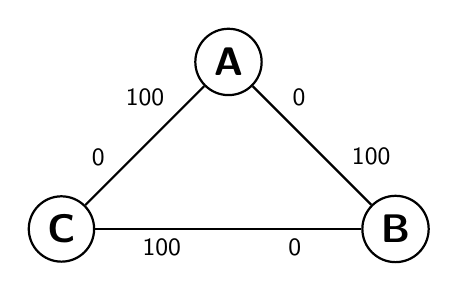
\begin{tikzpicture}[->,>=stealth',auto,node distance=3cm,
                    thick,main node/.style={circle,draw,font=\sffamily\Large\bfseries}]

  \node[main node] (A) {A};
  \node[main node] (B) [below right of=A] {B};
  \node[main node] (C) [below left of=A] {C};

  \draw[-, every node/.style={font=\sffamily\small}]
  	(A) edge node[near start] {0}
  			 node[near end] {100} (B)
  	(B) edge node[near start] {0}
  			 node[near end] {100} (C)
    (C)	edge node[near start] {0}
  			 node[near end] {100} (A)

  	;
\end{tikzpicture}
\caption{Simple skewed network. Each two parties share their own bi-directional payment channel. A's balances are 0 and 100 in its channels with B and C, respectively. B's balances are 100 and 0 with A and C respectively. C's balances are 100 and 0 with B and A, respectively.}
\label{skewed}
\end{figure}

Bi-directional payment channels can become highly skewed, and thus reduced to uni-directional channels, when used frequently to make transactions in one direction within the context of a payment routing network. Even though intermediate nodes that participate in the routing of a payment maintain their total balances, they are required to transfer the transacted amount from one payment channel to another.
As an example, a skewed network which could benefit from a rebalance of its ledgers is presented in Figure \ref{skewed}. In this simple case, even though A and B are connected by a direct payment channel, its balance is skewed in the direction of B. Therefore, if A wishes to make a transfer to B, the longer route comprised of A-C-B will have to be taken. This simple case can be generalized by considering the direct payment channel between A and B as some path that is shorter than the longer path from A through C to B.

If the intermediate nodes in a linked payment charge fees for routing the payment, then the skewness of the channels leads to an increased transaction cost because of the usage of longer paths in routing.
Moreover, in all aforementioned payment channel designs, the intermediate payment channels involved in a payment routing must freeze the transaction amount as collateral in order to guarantee the safe execution of the linked payment. In such a case, having to take longer paths because of skewness puts an increased collateral cost on payment routing.
In some situations, it could be considered beneficial for a payment channel that charges fees to offer negative routing fees in one direction as to promote that direction's use and cause the channel to be slowly rebalanced~\cite{negativefees}. Such a sacrificial strategy would become unnecessary in case \name is efficiently adopted.

\subsection{System Model}
Our rebalancing scheme is designed within the context of a decentralized blockchain that allows the trusted execution of smart contracts capable of supporting an off-chain payment network that contains a set of reasonably connected payment routers.

\subsubsection{Blockchain}
In our scheme, the blockchain is considered as an integrity protected and immutable root of trust that comprises a decentralized database containing a global view of accounts, their balances and transactions, and extra associated data.
Each account in the ledger is controlled by its own private key, that only the owner of the account should know. A transaction from any account cannot be authorized without possession of its respective private key.
Authorized modifications to the ledger are considered to be globally available after a block is generated, on average every predetermined block time T.

\subsubsection{Smart Contracts}
In addition to primitive ledger transactions that transfer balance from one account to another, our scheme also requires a smart contract execution environment, such as found in Ethereum~\cite{wood2014ethereum}.
Recall that Ethereum's smart contracts are allowed to hold a balance in the ledger, and control it according to their code.
We assume that once a smart contract is published, it cannot be modified, nor can a result outside the bounds of its correct execution be accepted on the global ledger.

\subsubsection{Off-chain Payment Network}
Our work is meant to be adapted to pre-existing off-chain payment network solutions to extend them with a safe rebalancing approach.
In our view of the system, we require the existence of an off-chain payment solution that allows a pair of peers to keep track of their own two-way ledgers off-chain. This off-chain ledger is assumed to be pegged to an on-chain smart contract that requires an initial funding from the two peers.
The contract is assumed to only allow peers to withdraw balances that they have both agreed on using their signatures. Of course, the sum of the two off-chain balances may not exceed the total deposit in the on-chain contract at any given time.

\subsubsection{Payment Network Topology}
The payment channel connectivity between the participants of a rebalancing is a core element to the efficacy of applying \name.
For a rebalancing to take place among a set of channel owners, each channel owner is expected to make a set of outgoing payments which are compensated by another set of incoming payments, through the same payment channels that connect the channel owners participating in a rebalancing.
This means that, when modeling the participants as nodes and the payment channels among them as edges, any such graph that contains no cycles\footnote{A sequence of vertices starting and ending at the same vertex.} is not rebalanceable. On the other hand, the more possible cycles present in the graph, the more potential rebalancing transactions there are to be found.

An example is presented in Figure~\ref{topologies}, whereby the network presented in Figure~\ref{topologies:a} contains no cycles and thus no rebalancing can take place, and the network presented in Figure~\ref{topologies:b} contains a few cycles that can be utilized. Moreover, all cycles can be utilized in parallel if the balances in the intersecting channels are sufficient. In Figure~\ref{topologies:b}, the channel between A and E appears in two such cycles, and the assumption when utilizing both cycles to enact a rebalancing is that E carries sufficient balance with A in that channel to compensate for the funds A gives to B and C.

\begin{figure}[h]
\centering

\begin{subfigure}[t]{0.45\columnwidth}
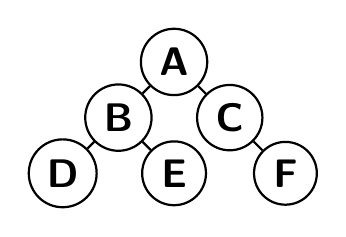
\begin{tikzpicture}[->,>=stealth',auto,node distance=1cm,
                    thick,main node/.style={circle,draw,font=\sffamily\Large\bfseries}]

  \node[main node] (A) {A};
  
  \node[main node] (B) [below left of=A] {B};
  \node[main node] (D) [below left of=B] {D};
  \node[main node] (E) [below right of=B] {E};
  
  \node[main node] (C) [below right of=A] {C};
  \node[main node] (F) [below right of=C] {F};
  

  \draw[-, every node/.style={font=\sffamily\small}]
  	(A) edge (B)
  	(A) edge (C)
  	
  	(B) edge (D)
  	(B) edge (E)
  	
  	(C) edge (F)

  	;
\end{tikzpicture}
\caption{An example network with a tree structure. Since no cycles exist in the graph, no viable rebalancing transactions can be found.}
\label{topologies:a}
\end{subfigure}
\hfill
\begin{subfigure}[t]{0.45\columnwidth}
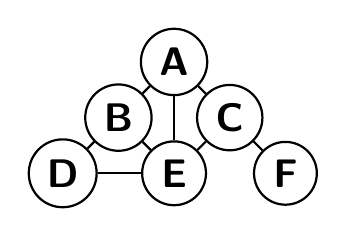
\begin{tikzpicture}[->,>=stealth',auto,node distance=1cm,
                    thick,main node/.style={circle,draw,font=\sffamily\Large\bfseries}]

  \node[main node] (A) {A};
  
  \node[main node] (B) [below left of=A] {B};
  \node[main node] (D) [below left of=B] {D};
  \node[main node] (E) [below right of=B] {E};
  
  \node[main node] (C) [below right of=A] {C};
  \node[main node] (F) [below right of=C] {F};
  

  \draw[-, every node/.style={font=\sffamily\small}]
  	(A) edge (B)
  	(A) edge (C)
  	
  	(B) edge (D)
  	(B) edge (E)
  	
  	(C) edge (F)
  	(C) edge (E)
  	
  	(D) edge (E)
  	
  	(E) edge (A)
  	;
\end{tikzpicture}
\caption{A example network containing cycles. Rebalancing payments can take paths such as: (A, B, D, E, A) and (C, E, B, D, E, A, C).}
\label{topologies:b}
\end{subfigure}

\caption{Example payment channel network topologies demonstrating when a rebalancing is possible.}
\label{topologies}
\end{figure}

\subsubsection{Communication Network}
For the purpose of the rebalancing scheme we assume an underlying communication network, where all the participants can communicate directly off-chain (e.g. via a TCP connection). Given that the participants had previously established off-chain payment channels, prior to needing to rebalance them, we assume that the line of communication that was used for channel establishment can be reused by our protocol.

\subsubsection{Adaptability}
%\todo{could you please elaborate why \name can be adapted to different payment networks? e.g. give example projects that would likely be adaptable.}
{\color{blue}
The algorithm for calculating a set of rebalancing transactions is independent from the enforcement mechanism of the transaction set. Therefore, to adapt \name to any blockchain satisfying our system model, one only needs to adapt the rebalancing protocol to support the target smart contract framework. For example, implementing the smart contracts provided in our paper for Ethereum \ref{sec:appendix:smartcontracts} in the Rootstock \cite{rootstock} smart contract platform for Bitcoin would provide the same on-chain enforcement mechanism required to settle disputes and atomically execute a transaction set. The off-chain peer to peer communications can then be directly made compliant.
}

\subsection{Rebalancing Protocol}
The protocol steps in Figure \ref{protocol} outline how the rebalancing group is expected to proceed in order to atomically execute a set of transactions.

\begin{figure}
    \centering
    \begin{sequencediagram}
        \newthread{ld}{Leader}
        \tikzstyle{inststyle}+=[below right=-0.83cm and 2cm of ld]
        \newinst{bc}{Blockchain}
        \tikzstyle{inststyle}+=[below right=-0.83cm and 2cm of bc]
        \newthread{pt}{Participant}
        
        
        \mess{pt}{Signal Rebalancing}{ld}
        \begin{call}{ld}{Rebalancing Init Req.}{pt}{Participation Confirmation}
        \end{call}
        
        \begin{call}{ld}{Channel Freeze Request}{pt}{\shortstack{
                Frozen Channels Confirmation \\
                Rebalance Objectives}}
            \postlevel
        \end{call}
                
        \begin{call}{ld}{Full Rebalancing Transaction Set}{pt}{Signed Commitment}
        \end{call}
        
        \mess{ld}{Full Signed Commitment Set}{pt}
        
        \mess{pt}{Dispute}{bc}
        
    \end{sequencediagram}
    \caption{Protocol Sequence Diagram. Solid lines with filled arrows require a response for the leader to proceed with the participant in the protocol. Dashed lines with arrow heads are the participant's responses. Solid lines with arrow heads do not require a response, and are not required for the sender or recipient to proceed.}
    \label{protocol}
\end{figure}

\subsubsection{Leader Election}
Before the protocol can commence, a leader needs to be elected to act as a point of synchronization for the protocol, and upon receiving enough information about channel balances, calculate a set of rebalancing transactions according to the specifications we discuss later. This leader does not need to be a stakeholder in any of the payment channels that are to be rebalanced, therefore, it may even be a third party chosen by the participants.

For our purposes, we adopt a leadership rotation strategy whereby all participants are identified by their public addresses in the global ledger, which we assume to be unique and numeric. We refer to the set of participants as $P$ and denote the public identifier of a participant $p \in P$ as $ID(p)$. Moreover, we assume that rebalancing rounds happen, among a fixed set of participants, in series. We refer to the point in time at which the participants formed a network that rebalances itself as $T_s$.

At $T_s$, the first leader is chosen as the participant p with the smallest identifier $ID(p)$ such that $\forall q\neq p \in P$:  $ID(p) < ID(q)$. After the completion of each round, or after a predefined amount of time passes since the termination of the last round, the next leader is chosen as the participant with the smallest identifier greater than that of the previous leader. More formally, the successor $s$ of a leader p, is the smallest such $s \in P$ so that $ID(s) > ID(p)$. If no such successor $s$ exists, then leadership is passed back to the first ever elected leader, which has the smallest identifier in the participant set.

In other cases, it might be preferable to allow only a subset of participants, perhaps even only one, to attain leadership due to, for example, their increased reliability or performance. \name can be adapted to any leader election strategy as the remaining protocol steps are decoupled from how the leader was chosen.


\subsubsection{Triggering}

At first, the currently elected leader waits for rebalancing initiation requests from participants in the sub-network. When enough requests are received (past an arbitrarily defined threshold), the leader sends an initiation request to all participants asking for confirmation of their participation in this round of rebalancing.
This triggering phase is customizable and serves to set a threshold past which a rebalancing is considered to be worth executing. This allows the protocol to scale its utility according to the size and requirements of the participants in a rebalancing group.

\subsubsection{Participation}
In response to the initialization request, the participants reply with a participation confirmation which allows the leader to construct a list of who will be partaking in rebalancing this round. This list is later on used to enable the safe execution of the rebalancing.
After receiving the confirmations, the leader announces to the involved participants which nodes are confirmed in the current round, and asks them to freeze the relevant payment channels they wish to rebalance.

\subsubsection{Transaction Set Generation}
Participants are then expected to respond with which channels they have frozen, along with their respective balances and objectives for the challenge. Mutual agreement by both owners of a payment channel on the freezing and the balances should be expected.
Moreover, the participants may submit rebalancing objectives, which specify whether they wish to gain or lose credit in each channel. Mutual agreement by both peers on the direction of rebalance in a channel should also be expected here. For example, if A wishes to gain credit in its channel with B, then B must be willing to lose credit in its channel with A.
The leader then proceeds to calculate a set of transactions that should conserve everyone's total balances, and abide by the participants' preferences for each channel. The generation is done through solving a linear program described below that produces a set of rebalancing transactions.

\subsubsection{Consensus}
The transaction set, along with a list of participating members, is then sent in the form of a commitment to all nodes for verification and signing. The commitment is composed of the merkle-tree root~\cite{Merkle1988} of all rebalancing transactions, and a hash of all the participants' public addresses (identities), both hashed together.
When participants receive this commitment from the leader, they verify the proper construction of the hashes, and that the rebalancing transactions are correctly generated. Each participant then responds to the leader with its own signature on the commitment.
Once all signatures are obtained by the leader, they are multicast to the involved participants. They can then consider the payment channels unfrozen, because the complete consensus on the transaction set can safely be considered as a binding state update for each payment channel.

\subsubsection{Dispute}
If the complete signature collection is withheld from some participant, it can issue an on-chain subsidized availability challenge for it. The response to that answer will be comprised of the complete rebalancing round data, which includes the set of participants, their signatures and the merkle root of the transaction set. If this challenge is not answered in some predefined amount of time, the rebalancing round is considered annulled, and participants can safely assume that the latest state prior to the rebalancing is valid. We discuss this issue in more detail in the security analysis presented in Section \ref{sec:analysis}.

\subsection{Rebalancing Objectives}
\label{objectives}

Participants can specify how they would like to shift the balances of their payment channels in a rebalancing instance, or an averaging method can be employed to automatically determine an equilibrium seeking set of objectives.

\subsubsection{Notation}
We denote the maximum balance shift that a node u is willing to sustain in its payment channel with a node v by $\Delta_{u,v}$
%, additionally when using a directional arrow, $\overrightarrow{\Delta_{u,v}} = X$ signifies that u is willing to lose a balance of X in the u-v payment channel, while $\overleftarrow{\Delta_{u,v}} = X$ would denote X as the balance u is looking to gain in the u-v payment channel.
, while $\delta_{u,v}$ denotes the balance that node u is going to gain in its payment channel with v as a result of the rebalancing transactions set.

\subsubsection{Linear Programming Model}
\label{linprog}

In our work, we model the rebalancing problem as a linear program. Several solving strategies for linear programs have been proposed and proven in various literature. We forgo a detailed examination of these methods and instead point the interested reader to sources such as~\cite{eiselt2007linear}, and the short discussion on linear programming in Section \ref{sec:relatedwork}.

The generation of a set of rebalancing transactions can be formulated as a linear program. In this model, participants may only specify for each channel a maximum amount they are willing to either gain or lose, but not both. If both peers of a payment channel agree on its direction of transfer, one variable denoting the positive direction of transfer is added to the linear program.\\

\noindent
\textbf{Linear Program:} Maximize: $\Sigma_{u,v} \delta_{u,v}$ Subject to:
%Maximize a linear function in O(N) variables subject to O(N) linear inequality constraints, where N is the number of payment channels.

\noindent
(1) $\forall u, v: \Delta_{u,v} > 0 \wedge \Delta_{v,u} < 0 \Leftrightarrow 0 \leq \delta_{u,v} \leq min(\Delta_{u,v}, -\Delta_{v,u}) $

\noindent
(2) $\forall u: \Sigma_{v} \delta_{v,u} = \Sigma_{v} \delta_{u,v} $\\

The objective of the linear program is to maximize the amount of funds moved between channels while the constraints serve to maintain the sanity and fairness of the generated transaction set.
The first constraint definition introduces linear constraints on the program as long as the two parties connected by the payment channel agree on the direction of balance change that they are willing to have in the channel. If A wishes to dispose of balance in the AB channel, and B wishes to gain balance in the same channel, then the $\delta_{a,b}$ variable is given an appropriate upper bound.
The second constraint enforces the conservation of balance, such that the set of resulting transactions is a zero sum rebalance, whereby no party gains or loses any money by executing the set of transactions relevant to its payment channels.

It is assumed that $\Delta_{u,v} \leq bal_{u,v}$ for all inputs $\Delta_{u,v}$ such that no payment channel is used past its total funding. It is also important that for any pair of (a,b), if $\delta_{a,b}$ is defined in the program, then $\delta_{b,a}$ is not, as that breaks the semantics of the constraints and the objective function.

\subsubsection{Channel Averaging Strategy}

In an automated setting where manual entry of rebalancing objectives is impractical, a strategy for automatically determining a set of objectives for each channel is required. To simplify the process of adopting our model in such a setting, we suggest the use of a straightforward strategy: averaging.
More formally, in this strategy, each two peers of a payment channel that is going to be rebalanced submit their rebalancing objectives as follows: $\forall u, v: \Delta_{u, v} = \frac{1}{2}(bal_u+bal_v) - bal_u$. This strategy can be followed using the linear model previously specified, since both peers would automatically agree on the direction of balance shift that seeks equilibrium.
We conjecture that this strategy, due to its nature, would improve the efficacy of a payment network after rebalancing in the average case. In cases where a channel imbalance in one direction is a favored outcome, then this strategy would lead to sub-optimal rebalances.

\subsubsection{Numerical Precision}

In all of the aforementioned solutions, the numerical accuracy of the program solving methods is a crucial detail to keep in mind. We do not employ integer programing methods for performance reasons, and allow fractional results to occur. Therefore, the resulting balance transfers from the linear program solution may very likely have a decimal precision beyond that of the underlying global ledger.
For this reason we resolve to simply rounding down the resulting transactions from our rebalancing schemes and assume that all losses incurred as a consequence are negligible. We justify this by examining the current smallest units that are exchangeable using Bitcoin and Ethereum, and their respective prices in US dollars as of the writing of this paper.

Until the writing of this paper, the maximum trading price of 1 Bitcoin is on the order of 1,000 U.S. dollars, while the smallest exchangeable unit, a satoshi, is equal to $10^{-8}$ Bitcoin. As for Ethereum, the maximum trading price as of yet is on the order of 100 U.S. dollars, while the smallest unit, wei, is equal to $10^{-18}$ Ether.
This puts the maximum possible loss incurred in each rebalancing transaction at a marginal fraction of a cent. If the trading values of these currencies at some point increase at least a million fold, then any non-integer solution would lead to some losses. However, we conjecture that if such an event occurs, then the global ledgers of these currencies will have to be extended to allow higher precision transactions, as to always be viable for micropayments and a realistic representation of monetary value.

\subsection{Optimality}
\label{optimality}
According to the rebalancing objectives defined in Section~\ref{objectives}, we defined the objective functions of the mathematical programming models to represent the total amount of funds shifted between payment channels, or, rebalanced. When using \name to improve the routing of future payments within a network, the optimal solution under such a definition would therefore be one that eliminates the most skewness in the network where possible.
For off-chain payment networks comprised of at least a few hundred payment routing nodes, it would be rather difficult to coordinate a successful global rebalancing where all network members are participants in a single \name rebalancing instance. Therefore, it would be more feasible to run multiple 'local' rebalances that ameliorate skewness in smaller sub-networks within the network in parallel.
More importantly, we conjecture that through running these multiple smaller instances, a globally optimal rebalancing can be approximated. We mainly base our argument on the expected outcome of running \name in multiple local instances on networks similar to the hypothetical network in topology in Figure~\ref{globalnetwork}.

\begin{figure}[htb!]
\centering
\begin{subfigure}[t]{0.45\columnwidth}
    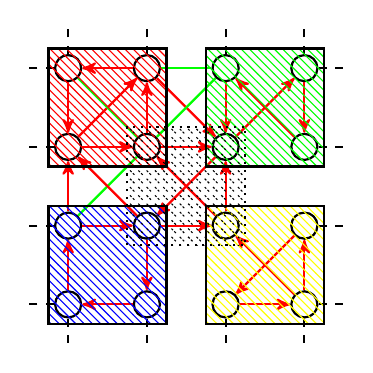
\begin{tikzpicture}[-,>=stealth',auto,thick,main node/.style={circle,draw,font=\sffamily\Large\bfseries}]
      \foreach \x in {0, ..., 3}
        \foreach \y in {0, ..., 3}
          \node [main node] (\x\y) at (\x,\y) {};
    
      %\foreach \x in {0, ..., 3}
      %  \foreach \y [count=\yi] in {0, ..., 2}
      %    \draw (\x\y) -- (\x\yi) (\y\x) -- (\yi\x);
      
      \draw[->, red] (00) -- (01);
      \draw[->, red] (01) -- (11);
      \draw[->, red] (10) -- (00);
      \draw[->, red] (11) -- (10);

      \draw[->, red] (03) -- (02);
      \draw[->, red] (02) -- (12);
      \draw[->, red] (02) -- (13);
      \draw[->, red] (12) -- (13);
      \draw[green] (12) -- (03);
      \draw[->, red] (13) -- (03);
      
      \draw[->, red] (22) -- (33);
      \draw[->, red] (23) -- (22);
      \draw[->, red] (33) -- (32);
      \draw[->, red] (32) -- (23);

      \draw[->, red] (20) -- (30);
      \draw[->, red] (30) -- (31);
      \draw[->, red] (31) -- (20);
      \draw[->, red] (30) -- (21);

      \draw[->, red] (11) -- (21);
      \draw[->, red] (21) -- (22);
      \draw[->, red] (22) -- (11);
      \draw[->, red] (12) -- (22);
      \draw[->, red] (21) -- (12);

      \draw[->, red] (01) -- (02);
      \draw[green] (01) -- (12);
      \draw[->, red] (11) -- (02);

      \draw[green] (13) -- (23);
      \draw[->, red] (13) -- (22);
      \draw[green] (12) -- (23);
          
      \foreach \i in {0, ..., 3} {
        \draw[-, dashed] ({\i3}) --++ (0,0.5cm);
        \draw[-, dashed] ({\i0}) --++ (0,-0.5cm);
        \draw[-, dashed] ({0\i}) --++ (-0.5cm,0);
        \draw[-, dashed] ({3\i}) --++ (0.5cm,0);
      }
      
      \draw[pattern=north west lines, pattern color=blue] (-0.25,-0.25) rectangle (1.25,1.25);
      \draw[pattern=north west lines, pattern color=red] (-0.25,1.75) rectangle (1.25,3.25);
      \draw[pattern=north west lines, pattern color=green] (1.75,1.75) rectangle (3.25,3.25);
      \draw[pattern=north west lines, pattern color=yellow] (1.75,-0.25) rectangle (3.25,1.25);
      \draw[pattern=north west lines, pattern color=black, dotted] (0.75,0.75) rectangle (2.25,2.25);


      
    \end{tikzpicture}
\caption{Example global network before local groups execute rebalances. There are five rebalancing groups in this figure: four in the corners, and one in the center.}
\end{subfigure}
\hfill
\begin{subfigure}[t]{0.45\columnwidth}
    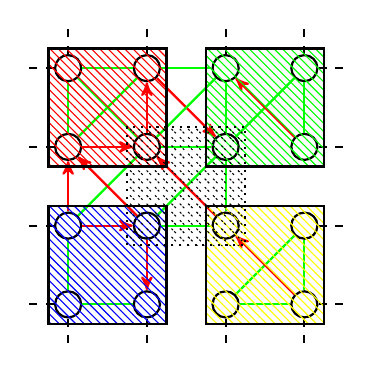
\begin{tikzpicture}[-,>=stealth',auto,thick,main node/.style={circle,draw,font=\sffamily\Large\bfseries}]
      \foreach \x in {0, ..., 3}
        \foreach \y in {0, ..., 3}
          \node [main node] (\x\y) at (\x,\y) {};
    
      %\foreach \x in {0, ..., 3}
      %  \foreach \y [count=\yi] in {0, ..., 2}
      %    \draw (\x\y) -- (\x\yi) (\y\x) -- (\yi\x);
      
      \draw[green] (00) -- (01);
      \draw[->, red] (01) -- (11);
      \draw[green] (10) -- (00);
      \draw[->, red] (11) -- (10);

      \draw[green] (03) -- (02);
      \draw[->, red] (02) -- (12);
      \draw[green] (02) -- (13);
      \draw[->, red] (12) -- (13);
      \draw[green] (12) -- (03);
      \draw[green] (13) -- (03);
      
      \draw[green] (22) -- (33);
      \draw[green] (23) -- (22);
      \draw[green] (33) -- (32);
      \draw[->, red] (32) -- (23);

      \draw[green] (20) -- (30);
      \draw[green] (30) -- (31);
      \draw[green] (31) -- (20);
      \draw[->, red] (30) -- (21);

      \draw[green] (11) -- (21);
      \draw[green] (21) -- (22);
      \draw[green] (22) -- (11);
      \draw[green] (12) -- (22);
      \draw[->, red] (21) -- (12);

      \draw[->, red] (01) -- (02);
      \draw[green] (01) -- (12);
      \draw[->, red] (11) -- (02);

      \draw[green] (13) -- (23);
      \draw[->, red] (13) -- (22);
      \draw[green] (12) -- (23);
          
      \foreach \i in {0, ..., 3} {
        \draw[-, dashed] ({\i3}) --++ (0,0.5cm);
        \draw[-, dashed] ({\i0}) --++ (0,-0.5cm);
        \draw[-, dashed] ({0\i}) --++ (-0.5cm,0);
        \draw[-, dashed] ({3\i}) --++ (0.5cm,0);
      }
      
      \draw[pattern=north west lines, pattern color=blue] (-0.25,-0.25) rectangle (1.25,1.25);
      \draw[pattern=north west lines, pattern color=red] (-0.25,1.75) rectangle (1.25,3.25);
      \draw[pattern=north west lines, pattern color=green] (1.75,1.75) rectangle (3.25,3.25);
      \draw[pattern=north west lines, pattern color=yellow] (1.75,-0.25) rectangle (3.25,1.25);
      \draw[pattern=north west lines, pattern color=black, dotted] (0.75,0.75) rectangle (2.25,2.25);
    \end{tikzpicture}
\caption{The same hypothetical network after the rebalancing groups conclude their local protocol runs.}
\end{subfigure}

\caption{Example effect of separate \name instances on a global network. Nodes in the graphs represent payment routers. Dashed edges represent terminal payment channels (e.g.\ to non-routing consumers). Green undirected edges represent balanced payment channels. Red directed edges represent skewed payment channels that allow payments in the edge direction. Shaded regions represent \name sub-networks.}
\label{globalnetwork}
\end{figure}

While a local, suboptimal solution may fail to rebalance as many payment channels as effectively as a global optimal solution would, the combination of multiple local \name solutions to global network would still lead to a more balanced global set of ledgers. Unless a very high degree of global coordination can be achieved, users of \name would have to make this trade-off in optimality. Moreover, even after a global run, some payment channels may remain skewed, because they could have significantly larger deposits in them than their peers' other payment channels, and thus there aren't enough funds to route to them.


\subsection{Atomic Enforceability}

For safety and efficiency purposes, we designed our protocol to use the underlying blockchain network primarily as a recourse. A valid rebalancing that results from the full execution of this protocol must be enforceable in the private payment channels involved, and thus also in the global decentralized ledger when need be. Likewise, an invalid rebalancing, should not be enforceable.

Payment channels are generally designed to support on-chain deposits and withdrawals of committed funds. Prior to finalizing withdrawals, the latest agreed upon balances of each channel peer must be broadcast on-chain in order to confirm that the amount to be withdrawn is correctly requested. Usually the state updates are modeled as a mutually signed commitment that reflects how much balance each peer of the payment channel has. In case the last agreed upon balances for the payment channel resulted from our rebalancing protocol, then the payment channel design must be extensible as to allow it to accept a valid rebalancing as yet another valid state update, even though its commitment structure would be different.

In \name (ref. Figure \ref{protocol}), the commitment sent back by participants encompasses the following two main elements: the full set of participants in this round, and the full set of rebalancing transactions that the leader has produced. Therefore, when a participant commits to a rebalancing round, it essentially authorizes that when the signatures of all the confirmed participants, in this round, are provided, for this round, then all of the payments included in the rebalancing transaction set are enforceable. This is done in order to mandate that all of the transactions in the rebalancing round are atomic, as in they will all proceed together or abort.

In retrospect, participants in a rebalancing agree to reduce some of the balances they are owed in some of their payment channels contingent on those losses being recovered as balance gains in other channels. Therefore, every participant must obtain a guarantee that all of their outgoing transactions are matched by some incoming transactions, and that if outgoing funds are enforceable, then incoming funds must also be enforceable to compensate. We designed our commitment scheme to account for these global enforceability reasons.

Moreover, broadcasting the data associated with a rebalancing on-chain to trigger a state update would always be more expensive than submitting a succinct, mutually signed balance commitment. We suggest an additional collaborative pre-broadcast step to alleviate this cost. After delivery of the full rebalancing signature set to both peers, they can simply mutually sign the transactions relevant to their mutual payment channels and send their respective signatures to each other.  While this step is purely optional and does not affect enforceability, it does allow peers to cut extra costs associated with performing on-chain withdrawals from a payment channel immediately following a rebalancing operation.

We demonstrate this concept by extending the Sprites~\cite{sprites} payment channel to accept a valid rebalancing, in addition to its regular two-party state update, as a valid balance commitment in our proof of concept implementation discussed in Section \ref{impl}.

%\subsubsection{Availability Disputes}
%A critical component to the enforceability of a rebalancing round is that the unanimous signature set collected by the leader be made available to every participant. In our design, prior to submitting a signed commitment, participants are sent the full round information that allows them to independently construct the commitment which they will sign.

\section{Security Analysis}
\label{sec:analysis}

Our protocol is designed to prevent any honest participant from losing any funds despite some strong adversarial assumptions. We will proceed to formally analyze the security guarantees of our protocol.
The global blockchain ledger acts as a recourse for dispute resolution, and there are costs associated with initiating and resolving these on-chain disputes. For example, a fee is paid per kilobyte of data broadcast on the Bitcoin blockchain~\cite{nakamoto2008bitcoin}, while gas is paid to activate smart contracts and enact transactions in Ethereum~\cite{buterin2014ethereum}. In our security analysis, we consider these expenses as external to the funds committed to in a rebalancing by participants. However, we also designed our protocol to minimize these expenses through requiring the least amount of information possible be needed on-chain in case of dispute.

\subsection{Threat Model}

We assume an irrational adversary that would be willing to lose some, or all, of their own comitted funds in order to cause honest parties to lose theirs, temporarily or otherwise. This irrational adversary may be in control of the leader role, some of the participants, or even all but one honest party that is the target of an attack.
An adversary in our model may cause parties under its control to sign and authorize any set of messages using their identities, or front-run any user input, but may not violate the integrity of the keys honest protocol participants use. In addition, we assume an adversary can cause denial of service attacks that abort the protocol at any given point.
In the following discussion, we define malicious behavior as that which would cause a participant committed to performing a set of transactions in a rebalancing to lose control of some or all of their committed funds, either permanently or temporarily.

\subsection{Guarantees for Honest Parties}

%\item Show that even against an irrational adversary, an honest participant cannot lose his funds (no matter how many participants are malicious).

Under the previous adversarial assumptions, a diligent honest participant in our protocol is able to protect itself from losing any of its committed funds, but will not be able to ensure that it is always treated fairly in the protocol or that the rebalancing always succeeds.

\subsubsection{Balance Conservation}
When the leader is done calculating a set of transactions that need to take place between participants in order to rebalance their payment channels, it then sends this set to each participant to commit to.
The information present in this set of transactions is sufficient for each honest party to decide whether the transaction set it is committing to will cause it to lose or gain any funds, because a diligent honest party should verify that all the transaction amounts related to its payment channels in the set sum up to a net total of zero\footnote{Up to the discussed numerical accuracy.}.
The most up to date state of a payment channel, where one is not a peer, cannot be truly verified unless broadcast onto a network. Each honest party can therefore only be responsible for verifying the balance conservation properties of transactions related to its payment channels.
This conservation check is sufficient to protect honest parties from committing to any rebalancing round that may cause them to lose funds. In case a set of transactions fails this check, then the honest party should not provide its signature. This effectively halts the rebalancing round as the full signed commitment set will never be producible by the adversary.

\subsubsection{Objective Satisfiability}

The protocol as we described it so far provides no guarantees towards fairness in rebalancing funds while equally satisfying the objectives set by all participants. A malicious leader may choose to omit, or restrict, the rebalancing objectives of some parties in order to produce a rebalancing set that is more favorable to the objectives of others, all while not violating the conservation of balance for any party. Unfairness may even arise from no malicious intent, but from the optimization path chosen by the linear program solver.
One approach might involve having the leader publicly commit to a randomness seed prior to requesting channel balance information. The leader then sends all initially received channel balances alongside the generated rebalancing transactions to each participant. Any participant interested would re-solve the linear program using the same seed of randomness in order to verify that the agreed upon objective function was indeed the one optimized for. Additionally, the transaction structure used in the payment channel must bind each new state to the previous one, so that the resulting rebalancing transactions are only enforceable if the correct balances were initially revealed.
This additional verification would of course come at the cost of the efficiency and privacy of the protocol, but that may be a critical trade-off an implementation of our protocol is inclined to make.

\subsubsection{Delayed Propagation Immunity}
\label{sec:analysis:dispute}
The adversary, whether in control of the leader, a subset of participants or just in control of the network, may opt to withhold, in one way or the other, the full signed commitment set from honest participants who wish to enforce the rebalancing transactions after having given their signed commitment.
Without the proper protection, this could lead to a dangerous situation whereby an enforceable state update to a payment channel is in the hands of the adversary and not the channel's honest owners. Effectively, this may lead an adversary that is in control of some of the direct peers of an honest participant, in addition to the leader, to steal committed funds.

Assuming that the adversary is in control of some of the direct peers of an honest participant, and that the channels between the honest participant and the adversary's participants are involved in the rebalancing, then the attack would proceed as follows:
The adversary would finalize the channels that have pending rebalancing transactions in favor of the honest participant and close them without honoring those transactions. Then the adversary would finalize the channels that have rebalancing transactions in favor of the honest participant's peers, but use the full commitment set to force the honoring of the pending transactions outgoing from the honest participant. In this case, the honest party loses the funds committed to the outgoing transactions in a rebalancing while not being able to claim the incoming funds.
One possibility would be to put an expiry date on the rebalancing, after which none of its transactions could be enforceable via an on-chain broadcast. However, this poses a problem to atomic enforceability, as some honest peers may have finalized their transactions before expiry, while other still haven't, due to network delays or otherwise. Another suggestion could be requiring that honest parties collaborate if any of them has received the full set. However, this is still not a formidable solution, as it is not effective when the adversary withholds the full set from all honest parties.

\paragraph{Solution}
Our proposed solution is to allow any participant to be able to issue an on-chain availability challenge towards the full signed commitment set. This challenge would carry an effective deadline by which the full signature set must be announced (by anyone) on-chain, or the rebalancing will be annulled and all of its transactions unenforceable in the global ledger.
One notable detail to take care of is that the grace period of channel finalization, as discussed in~\cite{sprites}, must be longer than the grace period extended by the availability challenge deadline as to effectively prevent the aforementioned attacks.
This solution imposes an added worst-case cost for running the protocol that increases proportionally to the number of participants involved in a single rebalancing. We discuss this issue further and provide some insights on how to possibly use \name in a reasonable manner as to minimize incurring worst-case costs in Section \ref{sec:usability}.

\subsubsection{Ungraceful Abortion}
If, from the view of an honest party, the protocol terminates at any point prior to the party's submission of its signature on the rebalancing commitment, then it is safe to assume that all the involved transactions are not enforceable.
However, termination of the protocol, for any reason, past the submission of the party's signature, and prior to its reception of the full signature set, is equivalent to the adversary withholding the signature set from the participant. In this case, as previously discussed in Section~\ref{sec:analysis:dispute}, the participant will need to issue the on-chain availability challenge.

\subsection{Privacy}

In order for the leader to effectively calculate the appropriate rebalancing transactions for the round, it must have knowledge of the latest balances of each involved payment channel. We consider this to be a privacy leaking component of the protocol equivalent to a public broadcast of the latest state of each involved payment channel.

In our adversarial setting, we hold no guarantees of what information may or may not be leaked by an adversary in control of the leader or any participant. Moreover, we note that the information carried in the structure of the transactions that are to be executed is highly dependant on the design of the underlying payment channel. For example, in our implementation using Sprites~\cite{sprites}, the leader is made aware of the last state of each participating payment channel, and then each participant is made aware of the next state of each payment channel after rebalancing.

On the other hand, in a payment channel design whereby the generated transaction set would not contain total balance information but rather balance changes, then only a malicious leader could cause a privacy leak. Malicious participants in this case would only learn changes in balances, but not what the starting or ending balances for each channel are, unless they are peers in them.

\section{Usability}
\label{sec:usability}

In this section we discuss the conditions under which \name would be suitable for use, its limitations and when it is advisable to employ.

\subsection{Context}

Employing off-chain solutions such as payment channels or other protocols (such as \name) implies a certain degree of trust between the involved parties. It is imperative, however, that trust be minimized wherever possible in a system design, and instead its trustworthiness increased.
In \name, when a party A agrees to participate in a rebalancing whereby another party, B, is participating, then A is effectively trusting that B will be available to not cause the protocol to abort prematurely. Moreover, if B is the acting leader in the round, then A is also trusting that B will not deny sending the full set of signatures to A.
These two expectations come at an operational risk. In the first case, A is only risking the collateral it has frozen for the protocol to proceed. If B causes the protocol to prematurely abort, then that collateral was frozen in vain when it could have been used elsewhere. In the second case, A is also risking being required to pay a fee for issuing an on-chain availability challenge for the signature set because of B's lack of cooperation.

For these reasons, we suggest that \name be employed in a context where the reliability of the involved peers is reputable in order to avoid needlessly tying collateral or incurring added costs repeatedly. We expect that payment routers that will face the problems \name aims to solve will be looking to establish relationships among each other that promote a functioning, reliable payment network. In the worst case, we have insured that no theft of committed funds is possible, but malfunctioning or malicious parties can still cause a denial, or degradation, of the service offered through \name.
We highly recommend utilizing \name in a reputation based context whereby participants are accountable for their previous reliability when running the protocol, and may be favored or dismissed in future rebalancing instances based on their attained reputation.

\subsection{Scaling and Associated Costs}

The design of \name centers around enabling a trust-free exchange of funds that rehabilitates a payment network and ensures that it is able to route payments efficiently. However, this trust-free design backed by a blockchain requires that in cases of dispute, enough non-repudiable information is available to decide a fair outcome.
A running instance of \name produces the minimal information needed to safely enable rebalancing, while ensuring that fund commitments are honored. As an instance grows in size, due to the participation of more users or the involvement of more payment channels, then more information is produced, which might make on-chain enforcement expensive or even impossible.
For this reason we offer advice on reasonably scaling up instances of \name, while not exceeding the limitations that a backing blockchain might have, using Ethereum as a practical example.

\subsubsection{Scaling Users}
\label{sec:usability:scale}
As more participants are involved in a rebalancing round, more signatures will need to be collected on the hash of the instance.
In Ethereum, the cost of verifying a user's signature on-chain in a smart contract is 3,000 gas units~\cite{buterin2014ethereum}. There are other costs associated with submitting data to a smart contract and processing it. In our implementation, discussed in Section~\ref{impl}, the cost of an on-chain dispute increases by approximately 9,000 gas units per involved participant. However, it is noteworthy to mention that in case Ethereum adopts the Schnorr \cite{Schnorr:1991:ESG:2724954.2725006} signature scheme (see Section \ref{sec:relatedwork}), this per user cost would drop by at least 4,400 gas\footnote{We base this estimate on the amount of data that would be spared from submission to the smart contract. We cannot estimate any further possible savings and we have no guarantee of how the implementation of this scheme might change other costs. } down to 4,600 (cf. Figure~\ref{savings}).
Recall the plot presented in Figure~\ref{savings}, which estimates the operational costs of naive on-chain rebalancing versus those of \name. 

\paragraph{Naive Transactions}
The worst case naive rebalancing would be if every user either withdraws or deposits into one of the involved payment channels. This would incur an Ethereum transaction cost of 21,000 gas~\cite{buterin2014ethereum} twice per channel, once by each peer. In the best case for naive rebalancing, each channel is only either deposited to, or withdrawn from, by one of its peers; therefore, the on-chain transaction cost is incurred only once per channel.

\paragraph{\name rebalancing}
In a flawless \name instance, where no disputes take place and everything is settled off-chain, there are exactly zero gas costs incurred, regardless of the number of channels involved.
As for the \name cost ranges, in the worst case, the rebalancing instance represents a ring network of users connected by payment channels, similar to that in Figure \ref{skewed}. Therefore, each additional payment channel adds a user to the instance, requiring an additional 9,000 gas units in disputes as discussed. In the best case of dispute, only two participants maintain all of the involved channels, which implies that only two signatures will ever be needed in case of dispute.\\

Ethereum has a mechanism which limits the amount of gas that can be exhausted per block~\cite{wood2014ethereum}, the gaslimit. Even if someone is willing to spend a considerable amount of ether to pay for the gas costs of verifying a large rebalancing instance, there still would be an upper bound that if reached, may render a rebalancing unverifiable on-chain, and thus unenforceable in practice.
In theory, on Ethereum, \name could be executed with roughly 300 participants and still produce verifiable instances. At a gas cost of 25 Gwei, such a rebalancing instance would cost approximately 0.075 Ether to verify. However, even when verifiability is not impossible, we very much advise against running the protocol at such a scale, unless a very high guarantee of reliability is available among participants.

Our recommendation is to calculate the estimated on-chain cost of verification prior to participating in a rebalancing, so that the risk of added running costs is known well ahead. Depending on the used blockchain, and the context of use, the costs and risks will vary, and should be estimated on a per use-case basis.

\subsubsection{Scaling Payment Channels}
Two peers may have more than one payment channel with each other. If we keep the number of participants in a rebalancing constant, we can add more payment channels to the rebalancing with an added cost per dispute that increases logarithmically in the number of involved channels. This is due to the use of merkle trees when constructing the rebalancing commitment. In case of dispute, the information required to be evaluated on-chain is comprised of participant signatures, and a merkle tree based proof of membership of a transaction in the transaction set. The merkle tree of transaction sets would grow in height logarithmically~\cite{Merkle1988} as more transactions are added, and thus the proof of membership would grow marginally longer.
Per Ethereum's implementation we estimate that the state update cost would grow by approximately 4,400 gas units per one level of height increase in the transaction set merkle tree.

\subsubsection{Linear Program Scalability}
Linear Program Solvers are highly efficient in practice. Even though some of their underlying algorithms may have exponential complexity in the worst-case, they were shown to converge in expected polynomial time of the number of variables~\cite{spielman2004smoothed}.
However, as efficient as these solvers are in practice, there is no absolutely guaranteed time by which they will terminate. As the problem size grows, the expected time towards reaching a solution increases. For this reason, users of \name must be mindful of the underlying limitations, since the linear programming model is the core of finding a satisfying set of rebalancing transactions.
Even when implemented over an underlying blockchain, or similar system, which has perfectly reliable participants and inexpensive on-chain dispute resolution, scaling the rebalancing instance to a significantly large number of payment channels, more than tens of thousands, may come at the cost of a very long time expenditure until the leader can generate a rebalancing, at least on an average desktop computer.
For this reason we suggest that the linear program instances be concerned with no more than a thousand payment channels, if not a few hundred, if such a demand were to arise and if the underlying blockchain would economically permit it (recall how dispute costs scale). If it is indeed found necessary to scale beyond that, then the participants should be split across several rebalancing instances, as at that scale the differences in optimality between global and local rebalances, as explained in \ref{optimality}, should be trivially inconsequential compared to the performance costs.

Besides our linear programming solution, other rebalancing objectives with more complex considerations could be explored. However, if the constraints become too complex, a non-linear solver might be required, which could render the process inefficient, or less scalable. We leave the exploration of further rebalancing objectives for future work.

\section{Proof of Concept Implementation}
\label{impl}
\todo{Link to Github Repository. Which license would you want to choose?}

To complement our protocol specification, we provide a working proof of concept, implemented in Python. The POC contains scripts that create a test blockchain network and some participants using the pyethereum library, on top of which our protocol is simulated. We also demonstrate how the mathematical model solutions can be translated into rebalancing transactions compatible with a modified version of the Sprites payment channel.

\subsection{Modified Sprites Payment Channel}
The first component of our implementation is a modified version of the Sprites~\cite{sprites} payment channel. Our modifications include two new features that are required for our protocol to proceed, and one additional security fix. In this section, we refer to the two source files written in the Solidity smart contract language, suffixed by '.sol'.

\subsubsection{Rebalance Challenge Contract}

The contract defined in 'challenge.sol' (cf. Appendix~\ref{sec:appendix:smartcontracts}) provides three main functionalities. The first of which is the ability to issue a subsidized availability challenge against a rebalancing instance. The issuer of the challenge must deposit an amount of funds that is proportional to the size of the rebalancing instance in order to pay for another party to respond to the challenge.
While this is an optional design choice, we determined the subsidization of the challenge to be the best course of action since it prohibits a malicious participant from issuing fake challenges with the intention of forcing one of the other nodes to pay to respond to it. Instead, now only in the case of a malicious leader would someone need to issue a challenge if the full signature set is not made available.
The second feature is the ability to permanently settle the availability and correctness of a rebalancing instance. This allows the instance to be used to update the on-chain state of any involved payment channel, closes any open challenges against it, and prohibits any future challenges from being issued.
The third feature is a simple check that allows any other smart contract, such as a payment channel contract, to verify whether a rebalancing instance has been verified for availability and correctness.

\subsubsection{Rebalance State Update}
Because the two parties responsible for a payment channel may not cooperatively sign the new state resulting from a valid rebalancing, the payment channel needs to be augmented so that it can accept a valid rebalancing, with full signatures, as a state update.
In 'channel.sol' (cf. Appendix~\ref{sec:appendix:smartcontracts}), we added a new functionality to the Sprites payment channel contract that allows a payment channel state to be updated on-chain after it has been verified in the rebalancing contract. After validation of the rebalancing instance, providing the signature of the counter-party in a payment channel on that instance, and the rebalancing transaction particular to the payment channel being updated, our modified contract accepts the new balances as the latest state.

\subsubsection{State Security Fix}
One final modification we made was the addition of the payment channel contract address to the state of the payment channel. The Sprites channel was constructed to accept an update state sent by one party if that party could provide the signature of the counter-party on that state. However, the state only contained a round number and balance information, but nothing that ties the state to one particular instance of a payment channel. Therefore, if a party were involved in multiple payment channels, their signature on the state of one of those channels could be used to update another channel as long as the on-chain deposits were not overdrawn by the update.

\subsection{Simulation Cases}
We present simulations of two different scenarios of mishaps that may occur in practice, and how to respond to them within the specification of the protocol while protecting user funds from being stolen.

\paragraph{Setup}
The simulations are initialized to reflect the example presented in Figure~\ref{skewed}, where three participants can use \name to rebalance their payment channels, such that the end goal of each participant is two channels with 50 credits in their favor, rather than one with 100 and the other with 0.

\subsubsection{On-chain Update}

In this case, referred to as test 'simulation\_scenario\_1', the protocol produces a valid rebalancing that is signed by everyone, and the signature set is made available to all participants for enforcement.
However, none of the participants choose to collaboratively sign the individual transactions within the rebalancing that are relevant to their payment channels. Therefore, they all resort to publishing and validating the rebalancing instance on-chain, and then using it to enforce a state update on their respective payment channel.
This case was designed to highlight the effect off-chain collaborative updates have on cutting expected running costs of the protocol.

\subsubsection{Availability Challenge}

In 'simulation\_scenario\_2', the full signature set is made unavailable for one of the participants. While a more mature implementation should include a means by which any participant can reach out to any other in order to request the full signature set if they have it, we simply highlight here that even in case one participant was isolated, they can still insure their funds.
The isolated participant proceeds to issue the availability challenge using the on-chain contract after having submitted their signature on the rebalancing instance and not getting a response. The main point that is highlighted here is that all honest parties are incentivized to answer the challenge, because it is subsidized, and in case the challenge expires the enforcement of their rebalancing transactions are voided if they have not yet locked in the transactions.
We postulate that as long as there remains one honest party with one payment channel with incoming funds not collaboratively finalized, then it is in their best interest to answer the posted challenge in order to secure their funds. This example also stresses that no two honest parties should collaboratively finalize a rebalancing transaction on their payment channel unless both have knowledge of the full signature set.

{\color{blue}A simulation of our model's effects over pre-existing transaction data from other sources would have further demonstrated its practicality. Unfortunately, we are limited in how much we can predict about the internal routing structures that would surface in real routing networks due to a lack of data from their relative novelty. Validating the simulation would therefore present a major obstacle.}

\subsection{Model Solution Interpretation}

In order to demonstrate how solutions to the mathematical models we have provided can be translated into practical transactions, in our case for the Sprites payment channel, we present an explanation of the definitions found in the 'linprog.py' python file.
The definition of 'linear\_program\_solution\_to\_transactions' is sufficient to translate the set of payment channel balance changes to a bundle of equivalent directional transactions.
The conversion is quite straightforward. If $\delta_{u,v}$ is positive then, as previously mentioned, funds should be transferred from u to v. In case of our sprites adaptation, we need to decrease the credits value of u, and increase that of v, in order to portray a transfer from u to v. The converse takes place if $\delta_{v,u}$ is negative.

\section{Related Work}
\label{sec:relatedwork}
In this section we survey related work.\\


\noindent
\textbf{Blockchain} Satoshi Nakamoto presented with the invention of Bitcoin in the year 2008~\cite{nakamoto2008bitcoin}, the first open and decentralized blockchain. Many alternative follow up blockchains have emerged since then, for example Ethereum~\cite{wood2014ethereum} which allows to express a richer transaction language through \emph{smart contracts}. Other proposals, such as zcash~\cite{sasson2014zerocash} and Monero~\cite{van2013cryptonote} have built up on Bitcoin to enhance the transaction privacy. Bonneau \emph{et al.}~\cite{bonneau2015sok} provide an excellent holistic overview of cryptocurrencies and related work in the field.
With the emergence of smart contracts and more expressive transaction languages, it was shown that smart contracts have severe security vulnerabilities~\cite{atzei2016survey}. Luu \emph{et al.}~\cite{luu2016making} provide a symbolic execution tool for current Ethereum smart contract developers to verify their code.
Schnorr signatures\cite{Schnorr:1991:ESG:2724954.2725006} have been recently suggested as a possible addition to Bitcoin\cite{scalingbitcoinschnorr}. This scheme allows the aggregation of multiple signatures into one which is verifiable against an aggregate of the relevant public keys in a single step. 
\\


\noindent
\textbf{Off-Chain Payment Networks:}
Several off-chain payment solutions have been proposed and can be divided into two categories. The first category relies on blockchain based \emph{timelocks} (e.g.\ by Decker \emph{et al.}~\cite{decker2015fast}). The channel starts with a committment transaction which for example lasts for 10 days. The subsequent commitment transaction will then last 9 days, and can thus be spent before the first transaction.
The second category of payment channels relies on punishment, i.e.\ if one party misbehaves, the other party can claim all funds of the channel. One instance of this payment channel is the Lightning Network\cite{lightning}. The Lightning Network relies on Bitcoin, while the Raiden Network\cite{raiden} is currently in development for the Ethereum blockchain.
Existing payment channels are still in early development and therefore allow for several improvement proposals. Sprites~\cite{sprites}, inspired by Lightning and Raiden aims to minimize the worst-case collateral costs of indirect off-chain payments. Flare~\cite{flare} is another proposal to optimize the search process of finding a payment route. Bolt~\cite{green2016bolt} provides different constructions that allow for privacy preserving off-chain payment channels. BitcoinJ, a lightweight Bitcoin client implementation, also supports micropayment channels~\cite{bitcoinj}.\\

\todo{any others that we should cite?}

\noindent
\textbf{Linear programming:}
Essentially, a mathematical programming model aims to represent a practical problem using numerical variables and parameters. While parameters are numbers that are known, or set, by the decision maker, the values of variables are to be determined in the process of solving the program.
In a linear program, a mathematical model may have linear (in)equality constraints that bound the possible values of the program variables. Moreover, there can also be a linear objective function which should be optimized for~\cite{dantzig1990origins}.

\paragraph{Linear Program Example:}
A simple linear program example is the following. Maximize: $F(x, y) = 2x - 3y$ Subject to:

\begin{enumerate}
    \item $120 \leq x \leq 210$
    \item $70 \leq y \leq 190$
    \item $250 \leq x + y$
\end{enumerate}

Solution: Max $F(x, y) = 210$ at $(x, y) = (210, 70)$

Linear programming has been a cornerstone of mathematical optimization problems since the introduction of the Simplex method by Dantzig in 1947~\cite{dantzig1990origins}. Even though its theoretical worse-case performance is exponential in the problem size, it has been found to be greatly efficient in practice, and has been widely adopted in numerous industrial fields~\cite{spielman2004smoothed}.
Interest developed into why an algorithm with very expensive worst-case performance costs was very successful and efficient in practice. The work presented in~\cite{spielman2004smoothed} analyzes the expected performance of the Simplex method in what is dubbed a smoothed analysis framework, and provides insight as to why the algorithm is quite successful despite its worst-case complexity.
Further works aimed to develop linear program solving methods that have better worst-case guarantees than those of Simplex. In 1978 Khachivan presented the first polynomial time algorithm for solving linear programs~\cite{khachiyan1980polynomial}, which achieved a worst case convergence time polynomial in the number of bits needed to represent the linear program. Despite its lower theoretical complexity compared to Simplex, the Ellipsoid method performed worse in practice~\cite{spielman2004smoothed}.
In the early 1980s, the interior point method was introduced by Karmakar~\cite{karmarkar1984new}. It is also guaranteed to converge in time polynomial in the linear problem size, but its practical performance has been on par with, and sometimes superior to, that of the simplex method~\cite{spielman2004smoothed}.


\section{Conclusion}
\label{sec:conclusion}
%The shape of future off-chain payment networks.
Decentralized blockchain ledgers that rely on miners to process transactions incentivize those miners with a reward for their contributions towards advancing the state of the global ledger. With the advent of off-chain payment networks, transaction processing will mostly be concerned with enacting changes to multiple private off-chain ledgers instead.
%Maintenance needs in credit balances and funding.
We have designed the \name protocol to maintain the equilibrium of the balances that intermediaries in a payment network keep among each other. Under ideal circumstances, this maintenance would come at no cost to the participants. This decreases undesirably long routing in case some of the payment channels in the network start attaining skewed balances.

%Blockchains and support for creating smart escrow contracts.
The core design of \name can be adapted to a decentralized ledger environment that allows the enforcement of one transaction, or lack thereof, to affect the enforcement of another. While we have found Ethereum, and Sprites, to be suitable environments in which to practically demonstrate \name, we encourage the adaptation of the protocol to other viable candidates.
%Rebalancing calculation methods. 
Our general method for generating a set of rebalancing transaction is based on solving a linear program. For the purpose of shifting the payment channel balances of \name participants towards equilibrium, we have provided an automatic way for establishing the required rebalancing objectives.

%Performance and scale.
Off-chain payment routing networks exhibit many challenges in terms of performance and scalability. For this reason we have provided a set of guidelines on how to safely adopt \name in a practical manner while minimizing exposure to potential performance penalties.

\section*{Acknowledgements}
This work was partly supported by the Zurich Information Security \& Privacy Center.

\bibliography{references}
\bibliographystyle{unsrt}

\section{Appendix}

\subsection{Blockchain Background}\label{sec:appendixblockchain}

\subsubsection{Blockchain Transactions}
Bitcoin transactions are sent from so-called addresses to other addresses. An address is a unique identifier (hash) of a public key. Only the owner of the correspondent private key is eligible to sign an appropriate transaction which allows to transfer monetary funds.

Interestingly, most currently proposed blockchains have a complex process for evaluating transactions in order to allow for a higher flexibility and extensibility of the application scenarios\footnote{Bitcoin transactions follow the unspent transaction output (UTXO) model, while Ethereum transactions are not UTXO based.}.

Bitcoin transactions are evaluated with a stack-based programming language called \emph{Script}. Mainly due to security reasons Script only supports a limited instruction set. The limited instruction set and the lack of an available high-level programming language have encouraged the development of blockchain systems supporting more intuitive and expressible programming languages. While there are several such systems (e.g., NXT, Clearmatics), Ethereum is the most popular one. Ethereum, was introduced in the year 2013 by Buterin~\cite{buterin2014ethereum}, and supports a pseudo\footnote{Pseudo, because the smart contract execution is halted if insufficient funds are provided for the execution, i.e.\ insufficient \emph{gas}.} Turing complete coding system. Its cryptocurrency is called ether and Ethereum supports two kinds of addresses: \emph{(i)} externally owned addresses (typically owned by a user) and \emph{(ii)} contract owned addresses. Ethereum programs run on the {Ethereum Virtual Machine} (EVM)~\cite{wood2014ethereum} and programs in EVM code are referred to as \emph{smart contracts}.

To avoid denial-of-service attacks, transactions are required to pay a fee for their execution. In Bitcoin, each transaction can pay a transaction fee, while in Ethereum, a transaction pays \emph{gas} (also to execute contracts).

\subsubsection{Smart Contracts}
Any Ethereum user is eligible to write and publish a smart contract (or contract). Other users can then execute the smart contract that is recorded in a block which is appended to the blockchain. Note that all information in the blockchain is publicly available.
To execute a contract, a user submits an Ethereum transaction containing all information required to process the contract. A miner can process the user transaction and commit it by writing this transaction to a new block (possibly along with other transactions). A valid block needs to be appended to the latest block of the blockchain\footnote{This is a simplification: miners ``compete'' on adding their own block to the top-most block of the blockchain until they reach a consensus on which miner has succeeded.}. A transaction is considered completed, when it has been added in a block. For security purposes, users should wait for several block confirmations (i.e., several additional blocks after the block containing the transaction), before considering a transaction to be final.


\subsection{Smart Contracts}\label{sec:appendix:smartcontracts}
In this section we provide the function signatures and main variables of our smart contracts.

\begin{lstlisting}[linewidth=\columnwidth,breaklines=true, caption={Smart contract defined in challenge.sol.}]
pragma solidity ^0.4.10;

contract RebalanceAvailabilityContract {
    function verifySignature(address pub, bytes32 h, uint8 v, bytes32 r, bytes32 s) {}

    function verifyAllSignatures(address[] pub, bytes32 h, uint8[] v, bytes32[] r, bytes32[] s) {}


    // Challenges can be answered within 5 blocks
    uint constant CHALLENGE_VALIDITY = 5;
    uint constant GAS_PRICE_IN_WEI = 25000000000 wei;
    // 2x sha3, storage value change, storage value load, transaction, data bytes
    uint constant GAS_PER_CHALLENGE_RESPONSE = 60 + 5000 + 200 + 21000 + 68*(32);
    // sha3(address), ecrecover, data bytes
    uint constant GAS_PER_PARTICIPANT = 6 + 3000 + 68*(1 + 32*2 + 20);

    mapping ( bytes32 => int ) challenge;

    // The issued challenge is subsidized by the participant who raises it.
    function submitChallenge(
            address[] participants,
            bytes32 transactionMerkleTreeRoot) payable {}

    function answerChallenge(
            uint8[] V,
            bytes32[] R,
            bytes32[] S,
            address[] participants,
            bytes32 transactionMerkleTreeRoot) {}

    function isChallengeSuccess(bytes32 instanceHash) returns(bool) {}
}    
\end{lstlisting}

\begin{lstlisting}[linewidth=\columnwidth,breaklines=true, caption={Smart contract defined in channel.sol. Adapted from the Sprites payment channel in \cite{sprites}.}]
pragma solidity ^0.4.10;

contract PaymentChannelRebalanceable {

    // Blocks for grace period
    uint constant DELTA = 10;

    // Events
    event EventInit();
    event EventUpdate(int r);
    event LogBytes32(bytes32 b);
    event LogAddress(address a);
    event LogInt(int i);
    event LogUInt(uint ui);
    event LogInts(int[2] i);
    event LogUInts(uint[2] ui);
    event LogBool(bool b);
    event EventPending(uint T1, uint T2);

    // Utility functions
    modifier onlyplayers {}
    function max(uint a, uint b) internal returns(uint) {}
    function min(uint a, uint b) internal returns(uint) {}
    function verifySignature(address pub, bytes32 h, uint8 v, bytes32 r, bytes32 s) {}
    function verifyMerkleChain(bytes32 link, bytes32[] chain, bool[] markleChainLinkleft) {}

    ///////////////////////////////
    // State channel data
    ///////////////////////////////
    int bestRound = -1;
    enum Status { OK, PENDING }
    Status public status;
    uint deadline;

    // Constant (set in constructor)
    address[2] public players;
    mapping (address => uint) playermap;
    RebalanceAvailabilityContract public rac;

    /////////////////////////////////////
    // Payment Channel - Application specific data
    ////////////////////////////////////

    // State channel states
    int [2] public credits;
    uint[2] public withdrawals;

    // Externally affected states
    uint[2] public deposits; // Monotonic, only incremented by deposit() function
    uint[2] public withdrawn; // Monotonic, only incremented by withdraw() function

    function sha3int(int r) constant returns(bytes32) {}

    function PaymentChannelRebalanceable(
            RebalanceAvailabilityContract _rac,
            address[2] _players) {}
        EventInit();
    }

    // Increment on new deposit
    function deposit() payable onlyplayers {}

    // Increment on withdrawal
    function withdraw() onlyplayers {}

    // State channel update function
    function update(uint[3] sig, int r, int[2] _credits, uint[2] _withdrawals)
            onlyplayers {}

    // State channel update function when latest change was due to rebalance
    function updateAfterRebalance(
            uint8[] V,
            bytes32[] R,
            bytes32[] S,
            address[] participants,
            bytes32[] transactionMerkleChain,
            bool[] markleChainLinkleft,
            int r,
            int[2] _credits,
            uint[2] _withdrawals)
                onlyplayers {}

    // State channel update function when latest change was due to rebalance
    function updateAfterRebalanceChallenged(
        address[] participants,
        bytes32[] transactionMerkleChain,
        bool[] markleChainLinkleft,
        int r,
        int[2] _credits,
        uint[2] _withdrawals)
            onlyplayers {}

    // Causes a timeout for the finalize time
    function trigger() onlyplayers {}

    function finalize() {}
}
\end{lstlisting}



\end{document}

